\documentclass{beamer}
\beamertemplatenavigationsymbolsempty
\usepackage{tikz}
\begin{document}
\begin{frame}
\centering
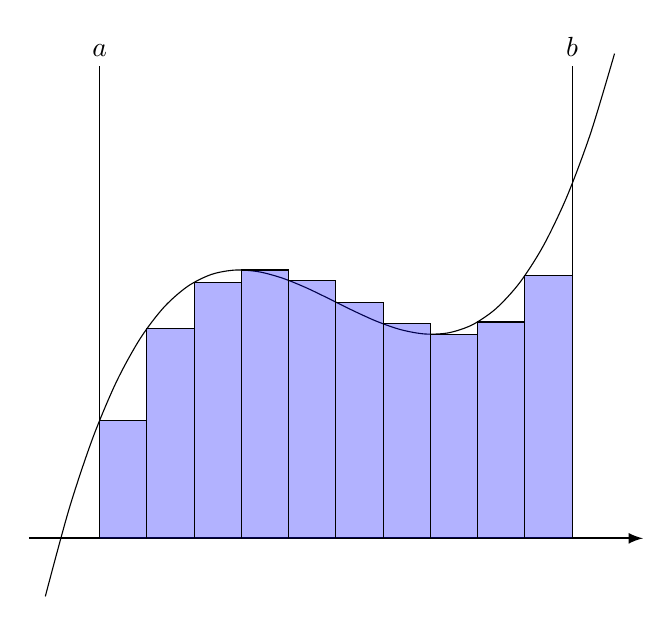
\begin{tikzpicture}[scale=3]
\draw[thick,-latex] (-1.3,0) -- (1.3,0);
%\draw[thick,-latex] (0,-0.3) -- (0,2.3);
\draw[domain=-1.23:1.18,smooth,variable=\Vt]
  plot (\Vt,{\Vt*\Vt*\Vt-0.5*\Vt+1},0);
\draw[] (-1,0) -- (-1,2) node[pos=1,above]{$a$};
\draw[] (1,0) -- (1,2) node[pos=1,above]{$b$};
\fill[blue, opacity=0.3] (-1.0,0) -- (-1.0,{-1.0^3-0.5*-1.0+1}) -- ++(0.2,0) |- (0,0);
\draw[] (-1.0,0) -- (-1.0,{-1.0^3-0.5*-1.0+1}) -- ++(0.2,0) |- (0,0);
\fill[blue, opacity=0.3] (-0.8,0) -- (-0.8,{-0.8^3-0.5*-0.8+1}) -- ++(0.2,0) |- (0,0);
\draw[] (-0.8,0) -- (-0.8,{-0.8^3-0.5*-0.8+1}) -- ++(0.2,0) |- (0,0);
\fill[blue, opacity=0.3] (-0.6,0) -- (-0.6,{-0.6^3-0.5*-0.6+1}) -- ++(0.2,0) |- (0,0);
\draw[] (-0.6,0) -- (-0.6,{-0.6^3-0.5*-0.6+1}) -- ++(0.2,0) |- (0,0);
\fill[blue, opacity=0.3] (-0.3999999999999999,0) -- (-0.3999999999999999,{-0.3999999999999999^3-0.5*-0.3999999999999999+1}) -- ++(0.2,0) |- (0,0);
\draw[] (-0.3999999999999999,0) -- (-0.3999999999999999,{-0.3999999999999999^3-0.5*-0.3999999999999999+1}) -- ++(0.2,0) |- (0,0);
\fill[blue, opacity=0.3] (-0.19999999999999996,0) -- (-0.19999999999999996,{-0.19999999999999996^3-0.5*-0.19999999999999996+1}) -- ++(0.2,0) |- (0,0);
\draw[] (-0.19999999999999996,0) -- (-0.19999999999999996,{-0.19999999999999996^3-0.5*-0.19999999999999996+1}) -- ++(0.2,0) |- (0,0);
\fill[blue, opacity=0.3] (0.0,0) -- (0.0,{0.0^3-0.5*0.0+1}) -- ++(0.2,0) |- (0,0);
\draw[] (0.0,0) -- (0.0,{0.0^3-0.5*0.0+1}) -- ++(0.2,0) |- (0,0);
\fill[blue, opacity=0.3] (0.20000000000000018,0) -- (0.20000000000000018,{0.20000000000000018^3-0.5*0.20000000000000018+1}) -- ++(0.2,0) |- (0,0);
\draw[] (0.20000000000000018,0) -- (0.20000000000000018,{0.20000000000000018^3-0.5*0.20000000000000018+1}) -- ++(0.2,0) |- (0,0);
\fill[blue, opacity=0.3] (0.40000000000000013,0) -- (0.40000000000000013,{0.40000000000000013^3-0.5*0.40000000000000013+1}) -- ++(0.2,0) |- (0,0);
\draw[] (0.40000000000000013,0) -- (0.40000000000000013,{0.40000000000000013^3-0.5*0.40000000000000013+1}) -- ++(0.2,0) |- (0,0);
\fill[blue, opacity=0.3] (0.6000000000000001,0) -- (0.6000000000000001,{0.6000000000000001^3-0.5*0.6000000000000001+1}) -- ++(0.2,0) |- (0,0);
\draw[] (0.6000000000000001,0) -- (0.6000000000000001,{0.6000000000000001^3-0.5*0.6000000000000001+1}) -- ++(0.2,0) |- (0,0);
\fill[blue, opacity=0.3] (0.8,0) -- (0.8,{0.8^3-0.5*0.8+1}) -- ++(0.2,0) |- (0,0);
\draw[] (0.8,0) -- (0.8,{0.8^3-0.5*0.8+1}) -- ++(0.2,0) |- (0,0);
\end{tikzpicture}
\end{frame}
\end{document}